\subsection{Bảo vệ dữ liệu tĩnh — AES-256-GCM}

\subsubsection{Mã hóa khóa bí mật của nút ký}

Khóa bí mật EC-Schnorr của mỗi nút ký ($d_i \in [1, n-1]$, biểu diễn 32 byte scalar) là tài sản nhạy cảm nhất trong toàn bộ hệ thống — nếu lộ ra, kẻ tấn công có thể tự sinh chữ ký hợp lệ thay cử tri. Khóa này \textbf{không bao giờ được lưu dưới dạng văn bản thuần}: trước khi ghi vào MongoDB, nó được mã hóa bằng AES-256-GCM với khóa đối xứng 32 byte cấp từ biến môi trường \texttt{ENCRYPTION\_KEY}. Hàm \texttt{encrypt} trong \texttt{libs/utils/crypto.util.ts} (Hình~\ref{fig:aes-gcm-encrypt}) thực hiện đúng năm bước: sinh IV ngẫu nhiên 12 byte, tạo \texttt{cipher} AES-256-GCM, mã hóa văn bản, lấy thẻ xác thực 16 byte, rồi ghép \textit{IV $\Vert$ AuthTag $\Vert$ Ciphertext} và mã hóa Base64.

\begin{figure}[H]
    \centering
    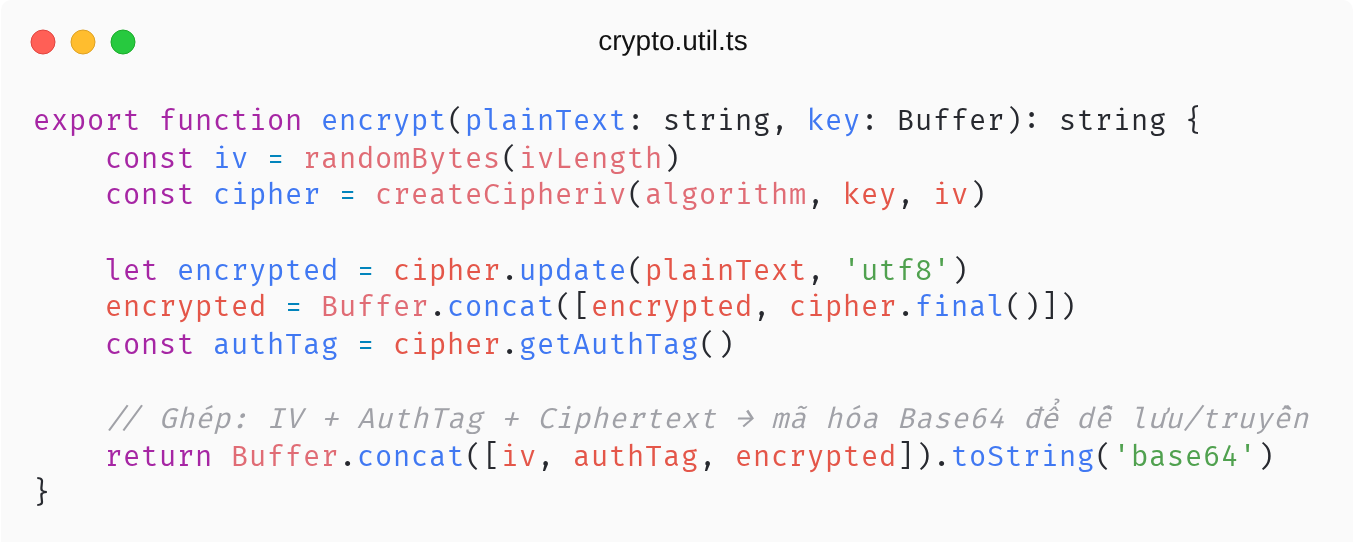
\includegraphics[width=0.85\textwidth, keepaspectratio]{Figures/code/aes-gcm-encrypt.png}
    \caption{Hàm mã hóa AES-256-GCM với IV ngẫu nhiên và thẻ xác thực}
    \label{fig:aes-gcm-encrypt}
\end{figure}

Pha giải mã bắt buộc gọi \texttt{decipher.setAuthTag(authTag)} trước khi \texttt{decipher.update} — nếu \textit{ciphertext} bị giả mạo dù chỉ một bit, phép xác thực thất bại và \texttt{decipher.final()} ném ngoại lệ. Bằng cách kiểm tra tính toàn vẹn ngay tại tầng mật mã, hệ thống phát hiện mọi sự xâm phạm vào dữ liệu khóa trong cơ sở dữ liệu — không phụ thuộc vào việc tin tưởng vào MongoDB hay tầng lưu trữ phía dưới.

\subsubsection{Vì sao chọn GCM thay vì CBC}

AES-256-GCM (\textit{Galois Counter Mode}) thuộc nhóm \textbf{Authenticated Encryption with Associated Data} (AEAD) — kết hợp mã hóa và xác thực trong cùng một phép biến đổi. So với AES-256-CBC (chế độ mã hóa khối truyền thống):

\begin{itemize}
    \item \textbf{Phát hiện giả mạo:} GCM sinh thẻ xác thực 16 byte gắn liền với ciphertext. CBC không có cơ chế này, dễ bị tấn công \textit{padding oracle} khi ciphertext bị thay đổi mà ứng dụng vẫn cố giải mã.

    \item \textbf{Bảo mật ngữ nghĩa (\textit{semantic security}):} IV ngẫu nhiên 12 byte ở mỗi lần mã hóa đảm bảo cùng một bản rõ luôn cho ciphertext khác nhau. Kẻ quan sát không thể suy ra mối quan hệ giữa các văn bản đã mã hóa.

    \item \textbf{Hiệu năng:} GCM hỗ trợ phần cứng AES-NI và tính toán song song theo \textit{counter mode}, nhanh hơn đáng kể so với CBC dạng tuần tự.
\end{itemize}

\subsubsection{Quản lý khóa mã hóa và vòng đời khóa bí mật}

\texttt{ENCRYPTION\_KEY} là 32 byte mã hóa Base64, được nạp từ biến môi trường khi dịch vụ khởi động. Trước khi sử dụng, hệ thống kiểm tra kích thước:

\begin{verbatim}
const encryptKeyBuf = Buffer.from(ENCRYPTION_KEY, 'base64')
if (encryptKeyBuf.length !== 32) {
    throw new BadGatewayException(
        'ENCRYPTION_KEY must be 32 bytes (256-bit) for AES-256')
}
\end{verbatim}

Nếu khóa sai kích thước, dịch vụ từ chối khởi động ngay lập tức thay vì \textit{im lặng} chạy với cấu hình yếu hơn. Tiếp cận \textit{fail-fast} này tránh tình huống nguy hiểm khi khóa bị cắt ngắn hay padding sai, hệ thống vẫn vận hành nhưng độ bảo mật thực tế đã giảm.

Trong bộ nhớ tiến trình, khóa bí mật $d_i$ chỉ tồn tại ngắn ngủi: nút ký nhận yêu cầu, đọc bản mã từ MongoDB, giải mã ra \texttt{bigint}, thực hiện phép tính $s_i = (k_i - d_i \cdot r) \bmod n$, rồi để biến \texttt{bigint} cho \textit{garbage collector} thu hồi. Hệ thống không log, không serialize, không truyền \textit{plaintext} của $d_i$ qua bất kỳ kênh giao tiếp nào. Cùng với việc xóa nonce $k_i$ ngay sau khi ký, đây là hai biện pháp đảm bảo \textit{key material} chỉ ở trong bộ nhớ trong cửa sổ thời gian tối thiểu cần thiết.
